We started out the project with a brainstorming session where we discussed different problems we would like to solve. By the end of the session, we came up with the following list of problems:
\begin{itemize}
	\item Noise pollution
	\item Navigation using echolocation
	\item Re-usability of heat waste
	\item Mapping of unknown terrains without any external technologies
	\item Maze navigation
\end{itemize}

We could identify a common theme amongst these problems, which led us to the conclusion that the problem domain should be within mapping and navigation. 

\begin{figure}[!h]
	\centering
	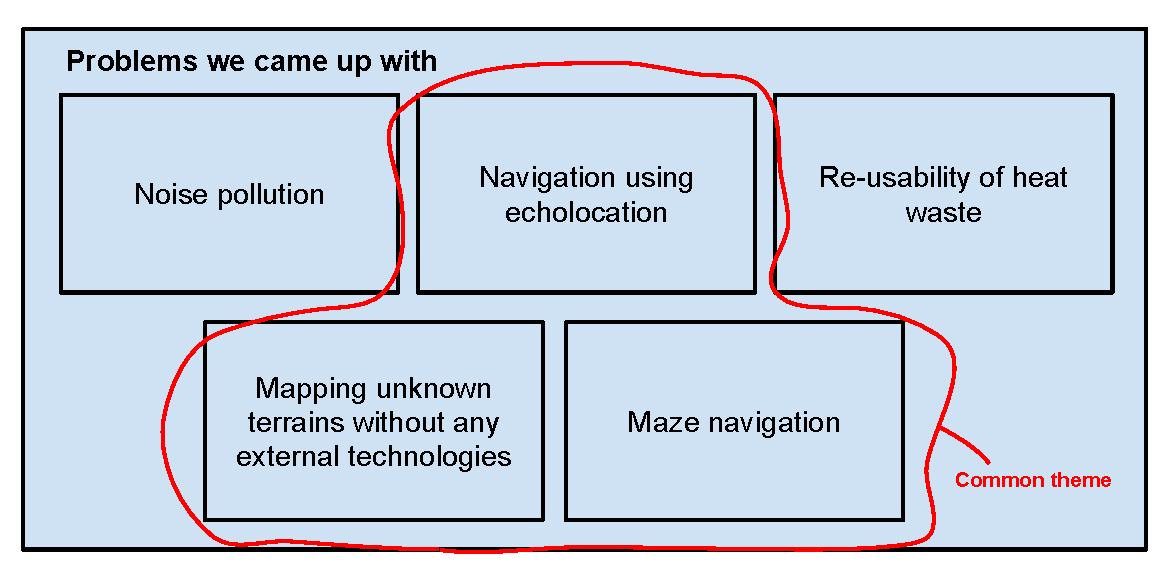
\includegraphics[scale=.7]{images/high-level-block.pdf}
	\caption{High-level block diagram expanding upon our brainstorming session}
	\label{fig:highlevelblock}
\end{figure}

Furthermore we decided to expand upon the problem-domain we set for ourselves and to deeper explore it. This led to more discussions on possible outcomes, uses and benefits of such system.

\begin{figure}[!h]
	\centering
	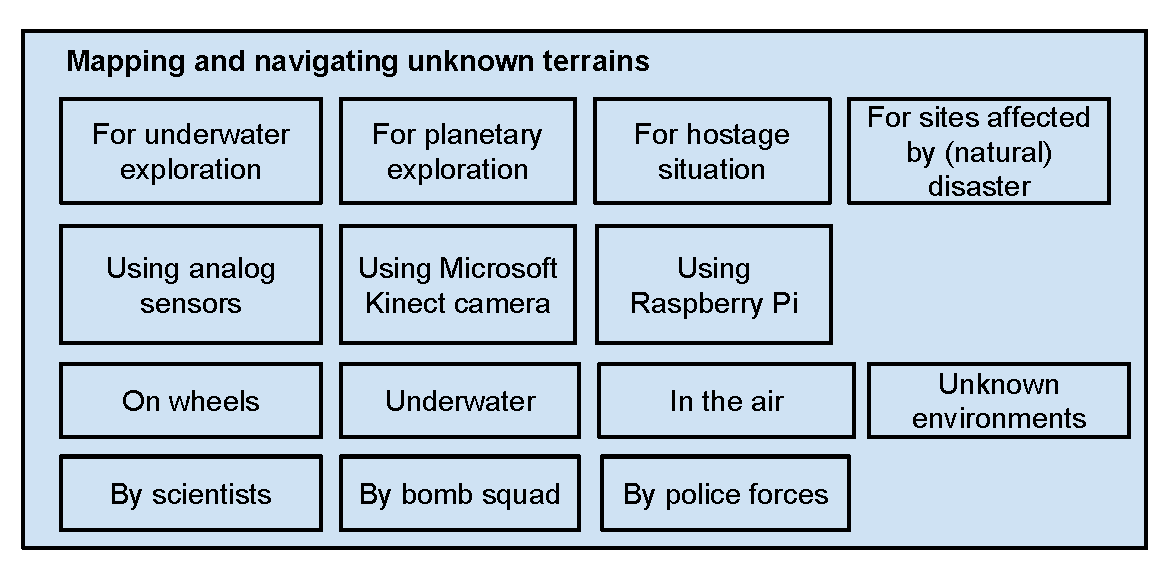
\includegraphics[scale=.7]{images/low-level-block.pdf}
	\caption{Low-level block diagram expanding upon the common theme we found}
	\label{fig:lowlevelblock}
\end{figure}

We decided to continue on with the selected problem-domain and started using a W-diagram model to expand upon it further and to identify the parts needed to be researched. This method will help us to come up with a solution to the problem at hand.